
\begin{multicols}{2}
Vers 200 Avant J.C., le mathématicien astronome grec \'Eratosthène avait utilisé les remarques suivantes :
\begin{enumerate}
\item[\ding{172}] En un point $A$ de la haute vallée du Nil (Syène, aujourd'hui Assouan), le soleil éclaire un certain jour à midi le fond des puits, il est dont à la verticale du point $A$.
\item[\ding{173}] Au même instant, en un point $B$ du delta du Nil 
(Alexandrie) (c'est-à-dire situé sur le même méridien que $A$); le soleil fait avec la verticale un angle $\alpha$ qu'un observateur peut relever.
\item[\ding{174}] Comme le soleil est très loin, on peut considérer que les droites qui vont de $A$ au soleil et de $B$ au soleil sont pratiquement parallèles.
\end{enumerate}
\begin{enumerate}
  \item Explique comment, connaissant la distance de $A$ à $B$ et l'angle $\alpha$, Eratosthène a pu calculer (approximativement) le rayon de la Terre.
\item Evalue à ton tour le rayon de la Terre sachant que $AB=800$~km et $\alpha=7\degres$.
\end{enumerate}
 
 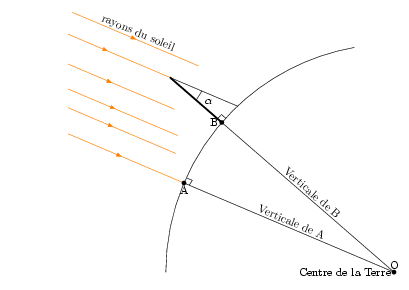
\includegraphics[scale=1]{TR-217.png}  
  \end{multicols}